% questions.tex —— 2010 年·普通高等学校招生考试·北京卷·文科 · 题目内容片段（无答案）
% 由 tools/generate_projects.py 依来源总账自 2010/2010_数学真题_北京文_试题.md 生成，勿手改（改源 MD 后重跑）


状态：needs-review；依固定候选 PDF 两页（印刷页 575–576）逐题核验，七幅图已矢量重绘。原页未印分值，不补。

\gkpart{一、选择题}

\begin{question}
\gkti{1}集合 $P=\{x\in\mathbf Z\mid0\leqslant x<3\}$，$M=\{x\in\mathbf Z\mid x^2\leqslant9\}$，则 $P\cap M=$（　）

（A）$\{1,2\}$

（B）$\{0,1,2\}$

（C）$\{1,2,3\}$

（D）$\{0,1,2,3\}$

\end{question}
\begin{question}
\gkti{2}在复平面内，复数 $6+5\mathrm i$，$-2+3\mathrm i$ 对应的点分别为 $A$，$B$。若 $C$ 为线段 $AB$ 的中点，则点 $C$ 对应的复数是（　）

（A）$4+8\mathrm i$

（B）$8+2\mathrm i$

（C）$2+4\mathrm i$

（D）$4+\mathrm i$

\end{question}
\begin{question}
\gkti{3}从 $\{1,2,3,4,5\}$ 中随机选取一个数为 $a$，从 $\{1,2,3\}$ 中随机选取一个数为 $b$，则 $b>a$ 的概率是（　）

（A）$\dfrac45$

（B）$\dfrac35$

（C）$\dfrac25$

（D）$\dfrac15$

\end{question}
\begin{question}
\gkti{4}若 $\boldsymbol a$，$\boldsymbol b$ 是非零向量，且 $\boldsymbol a\perp\boldsymbol b$，$|\boldsymbol a|\neq|\boldsymbol b|$，则函数 $f(x)=(x\boldsymbol a+\boldsymbol b)\cdot(x\boldsymbol b-\boldsymbol a)$ 是（　）

（A）一次函数且是奇函数

（B）一次函数但不是奇函数

（C）二次函数且是偶函数

（D）二次函数但不是偶函数

\Needspace{0.4\textheight}
\end{question}
\begingroup
\renewenvironment{question}{\Needspace{0.5\textheight}}{}
\begin{question}
\gkti{5}一个长方体去掉一个小长方体，所得几何体的正（主）视图与侧（左）视图分别如图所示，则该几何体的俯视图为（　）
\nopagebreak[4]
\begin{center}% 2010 年北京卷文科第 5 题：正视图、侧视图与四个俯视图选项。
% 来源 PDF：普通高考/2010/2010北京文.pdf，SHA-256 8def639c25748266a140a99f6111811c7037bced389a451089eff7b1a0b0ba52。
% 原页：第 1 页（A3 三栏）第 1 栏中部，书页码 575。
\begin{tikzpicture}[semithick, every node/.style={inner sep=1.2pt, font=\small}]
  % 正视图
  \draw (0,0) rectangle (1.6,1.0);
  \draw (0,0.6) -- (0.6,0.6) -- (0.6,1.0);
  \node[below] at (0.8,-0.1) {正（主）视图};
  % 侧视图
  \draw (2.4,0) rectangle (4.0,1.0);
  \draw (2.4,0.6) -- (3.4,0.6) -- (3.4,1.0);
  \node[below] at (3.2,-0.1) {侧（左）视图};
  % 四个俯视图选项
  \draw (0,-2.0) rectangle (1.6,-0.8);
  \draw (0.6,-2.0) -- (0.6,-1.4) -- (1.6,-1.4);
  \node[below] at (0.8,-2.1) {（A）};
  \draw (2.4,-2.0) rectangle (4.0,-0.8);
  \draw (2.4,-1.4) -- (3.4,-1.4) -- (3.4,-0.8);
  \node[below] at (3.2,-2.1) {（B）};
  \draw (0,-3.6) rectangle (1.6,-2.4);
  \draw (0,-3.0) -- (0.6,-3.0) -- (0.6,-2.4);
  \node[below] at (0.8,-3.7) {（C）};
  \draw (2.4,-3.6) rectangle (4.0,-2.4);
  \draw (3.4,-3.6) -- (3.4,-3.0) -- (4.0,-3.0);
  \node[below] at (3.2,-3.7) {（D）};
\end{tikzpicture}
\end{center}
\nopagebreak[4]
\end{question}
\endgroup
\begin{question}
\gkti{6}给定函数：① $y=x^{\frac12}$，② $y=\log_{\frac12}(x+1)$，③ $y=|x-1|$，④ $y=2^{x+1}$，其中在区间 $(0,1)$ 上单调递减的函数序号是（　）

（A）①②

（B）②③

（C）③④

（D）①④

\Needspace{0.4\textheight}
\end{question}
\begingroup
\renewenvironment{question}{\Needspace{0.5\textheight}}{}
\begin{question}
\gkti{7}某班设计了一个八边形的班徽（如图），它由腰长为 $1$、顶角为 $\alpha$ 的四个等腰三角形，及其底边构成的正方形所组成，该八边形的面积为（　）

（A）$2\sin\alpha-2\cos\alpha+2$

（B）$\sin\alpha-\sqrt3\cos\alpha+3$

（C）$\sqrt3\sin\alpha-\sqrt3\cos\alpha+1$

（D）$2\sin\alpha-\cos\alpha+1$
\nopagebreak[4]
\begin{center}% 2010 年北京卷文科第 7 题：八边形班徽（四个腰长为 1、顶角为 α 的等腰三角形 + 正方形）。
% 来源 PDF：普通高考/2010/2010北京文.pdf，SHA-256 8def639c25748266a140a99f6111811c7037bced389a451089eff7b1a0b0ba52。
% 原页：第 1 页（A3 三栏）第 1 栏下部，书页码 575。
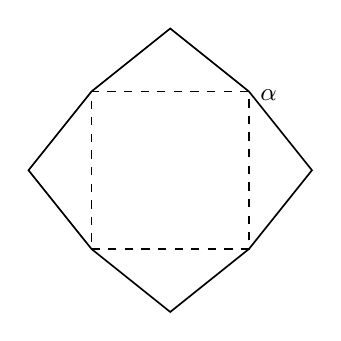
\begin{tikzpicture}[semithick, every node/.style={inner sep=1.2pt, font=\small}]
  % 正方形
  \coordinate (A) at (-1,-1);
  \coordinate (B) at (1,-1);
  \coordinate (C) at (1,1);
  \coordinate (D) at (-1,1);
  \draw[dashed] (A) -- (B) -- (C) -- (D) -- cycle;
  % 四个等腰三角形的外顶点
  \coordinate (P1) at (0,1.8);
  \coordinate (P2) at (1.8,0);
  \coordinate (P3) at (0,-1.8);
  \coordinate (P4) at (-1.8,0);
  \draw (D) -- (P1) -- (C);
  \draw (C) -- (P2) -- (B);
  \draw (B) -- (P3) -- (A);
  \draw (A) -- (P4) -- (D);
  \node at (1.25,0.95) {$\alpha$};
\end{tikzpicture}
\end{center}
\nopagebreak[4]
\Needspace{0.4\textheight}
\end{question}
\endgroup
\begingroup
\renewenvironment{question}{\Needspace{0.5\textheight}}{}
\begin{question}
\gkti{8}如图，正方体 $ABCD-A_1B_1C_1D_1$ 的棱长为 $2$，动点 $E$，$F$ 在棱 $A_1B_1$ 上，点 $Q$ 是棱 $CD$ 的中点，动点 $P$ 在棱 $AD$ 上，若 $EF=1$，$DP=x$，$A_1E=y$（$x,y$ 大于零），则三棱锥 $P-EFQ$ 的体积（　）

（A）与 $x$，$y$ 都有关

（B）与 $x$，$y$ 都无关

（C）与 $x$ 有关，与 $y$ 无关

（D）与 $y$ 有关，与 $x$ 无关
\nopagebreak[4]
\begin{center}% 2010 年北京卷文科第 8 题：正方体 ABCD-A1B1C1D1，E、F 在 A1B1 上，P 在 AD，Q 为 CD 中点。
% 来源 PDF：普通高考/2010/2010北京文.pdf，SHA-256 8def639c25748266a140a99f6111811c7037bced389a451089eff7b1a0b0ba52。
% 原页：第 1 页（A3 三栏）第 2 栏上部，书页码 575。
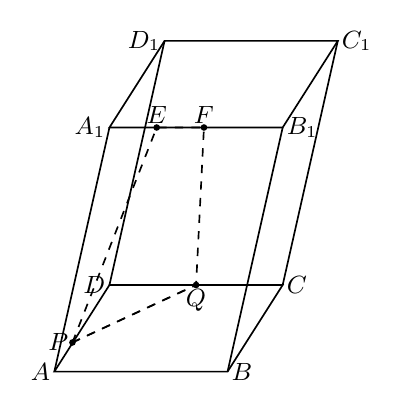
\begin{tikzpicture}[semithick, every node/.style={inner sep=1.2pt, font=\small}]
  \coordinate (A) at (0,0);
  \coordinate (B) at (2.2,0);
  \coordinate (C) at (2.9,1.1);
  \coordinate (D) at (0.7,1.1);
  \coordinate (A1) at (0.7,3.1);
  \coordinate (B1) at (2.9,3.1);
  \coordinate (C1) at (3.6,4.2);
  \coordinate (D1) at (1.4,4.2);
  % 可见棱
  \draw (A) -- (B) -- (C) -- (D) -- cycle;
  \draw (A) -- (A1);
  \draw (B) -- (B1);
  \draw (C) -- (C1);
  \draw (D) -- (D1);
  \draw (A1) -- (B1) -- (C1) -- (D1) -- cycle;
  % E、F 在 A1B1 上
  \coordinate (E) at (1.3,3.1);
  \coordinate (F) at (1.9,3.1);
  % P 在 AD 上，Q 为 CD 中点
  \coordinate (P) at (0.23,0.37);
  \coordinate (Q) at (1.8,1.1);
  \fill (E) circle (1.2pt);
  \fill (F) circle (1.2pt);
  \fill (P) circle (1.2pt);
  \fill (Q) circle (1.2pt);
  \draw[dashed] (P) -- (E) -- (F) -- (Q) -- cycle;
  \draw[dashed] (P) -- (Q);
  % 标注
  \node[left] at (A) {$A$};
  \node[right] at (B) {$B$};
  \node[right] at (C) {$C$};
  \node[left] at (D) {$D$};
  \node[left] at (A1) {$A_1$};
  \node[right] at (B1) {$B_1$};
  \node[right] at (C1) {$C_1$};
  \node[left] at (D1) {$D_1$};
  \node[above] at (E) {$E$};
  \node[above] at (F) {$F$};
  \node[left] at (P) {$P$};
  \node[below] at (Q) {$Q$};
\end{tikzpicture}
\end{center}
\nopagebreak[4]
\end{question}
\endgroup
\gkpart{二、填空题}

\Needspace{0.4\textheight}
\begingroup
\renewenvironment{question}{\Needspace{0.5\textheight}}{}
\begin{question}
\gkti{9}已知函数 $y=\begin{cases}\log_2x,&x\geqslant2,\\ 2-x,&x<2.\end{cases}$ 如图表示的是给定 $x$ 的值，求其对应的函数值 $y$ 的程序框图。① 处应填写$\underline{\qquad}$；② 处应填写$\underline{\qquad}$。
\nopagebreak[4]
\begin{center}% 2010 年北京卷文科第 9 题：分段函数程序框图。
% 来源 PDF：普通高考/2010/2010北京文.pdf，SHA-256 8def639c25748266a140a99f6111811c7037bced389a451089eff7b1a0b0ba52。
% 原页：第 1 页（A3 三栏）第 2 栏中部，书页码 575。
\begin{tikzpicture}[semithick, every node/.style={inner sep=2pt, font=\small}, >=stealth]
  \node[draw,rounded corners] (start) at (0,0) {开始};
  \node[draw,rectangle] (in) at (0,-1.1) {输入 $x$};
  \node[draw,diamond,aspect=2] (test) at (0,-2.4) {①};
  \node[draw,rectangle] (no) at (2.2,-2.4) {②};
  \node[draw,rectangle] (yes) at (0,-3.7) {$y=2-x$};
  \node[draw,rectangle] (out) at (1.1,-5.0) {输出 $y$};
  \node[draw,rounded corners] (end) at (1.1,-6.1) {结束};
  \draw[->] (start) -- (in);
  \draw[->] (in) -- (test);
  \draw[->] (test) -- node[above] {是} (yes);
  \draw[->] (test) -- node[above] {否} (no);
  \draw[->] (yes) -- (out);
  \draw[->] (no) |- (out);
  \draw[->] (out) -- (end);
\end{tikzpicture}
\end{center}
\nopagebreak[4]
\end{question}
\endgroup
\begin{question}
\gkti{10}在 $\triangle ABC$ 中，若 $b=1$，$c=\sqrt3$，$\angle C=\dfrac{2\pi}3$，则 $a=$ $\underline{\qquad}$。

\end{question}
\begin{question}
\gkti{11}若点 $P(m,3)$ 到直线 $4x-3y+1=0$ 的距离为 $4$，且点 $P$ 在不等式 $2x+y<3$ 表示的平面区域内，则 $m=$ $\underline{\qquad}$。

\Needspace{0.4\textheight}
\end{question}
\begingroup
\renewenvironment{question}{\Needspace{0.5\textheight}}{}
\begin{question}
\gkti{12}从某小学随机抽取 $100$ 名同学，将他们的身高（单位：厘米）数据绘制成频率分布直方图（如图）。由图中数据可知 $a=$ $\underline{\qquad}$。若要从身高在 $[120,130)$，$[130,140)$，$[140,150]$ 三组内的学生中，用分层抽样的方法选取 $18$ 人参加一项活动，则从身高在 $[140,150]$ 内的学生中选取的人数应为$\underline{\qquad}$。
\nopagebreak[4]
\begin{center}% 2010 年北京卷文科第 12 题：频率分布直方图。
% 来源 PDF：普通高考/2010/2010北京文.pdf，SHA-256 8def639c25748266a140a99f6111811c7037bced389a451089eff7b1a0b0ba52。
% 原页：第 1 页（A3 三栏）第 3 栏中部，书页码 575。
\begin{tikzpicture}[semithick, x=0.9cm, y=28cm, every node/.style={inner sep=1.2pt, font=\small}]
  \draw[-stealth] (0,0) -- (5.6,0) node[below] {身高};
  \draw[-stealth] (0,0) -- (0,0.04) node[left] {$\dfrac{\text{频率}}{\text{组距}}$};
  \foreach \i/\h/\lab in {0/0.005/,1/0.035/,2/0.030/a,3/0.020/,4/0.010/}{
    \draw[fill=gray!15] (\i,0) rectangle (\i+0.9,\h);
    \node[above] at (\i+0.45,\h) {$\lab$};
  }
  \foreach \i/\t in {0/100,1/110,2/120,3/130,4/140,5/150}{
    \node[below] at (\i,0) {\t};
  }
\end{tikzpicture}
\end{center}
\nopagebreak[4]
\end{question}
\endgroup
\begin{question}
\gkti{13}已知双曲线 $\dfrac{x^2}{a^2}-\dfrac{y^2}{b^2}=1$（$a>0$，$b>0$）的离心率为 $2$，焦点与椭圆 $\dfrac{x^2}{25}+\dfrac{y^2}9=1$ 的焦点相同，那么双曲线的焦点坐标为$\underline{\qquad}$；渐近线方程为$\underline{\qquad}$。

\Needspace{0.4\textheight}
\end{question}
\begingroup
\renewenvironment{question}{\Needspace{0.5\textheight}}{}
\begin{question}
\gkti{14}如图放置的边长为 $1$ 的正方形 $PABC$ 沿 $x$ 轴滚动。设顶点 $P(x,y)$ 的纵坐标与横坐标的函数关系是 $y=f(x)$，则 $f(x)$ 的最小正周期为$\underline{\qquad}$；$y=f(x)$ 在其两个相邻零点间的图象与 $x$ 轴所围区域的面积为$\underline{\qquad}$。

说明：“正方形 $PABC$ 沿 $x$ 轴滚动”包括沿 $x$ 轴正方向和沿 $x$ 轴负方向滚动。沿 $x$ 轴正方向滚动指的是先以顶点 $A$ 为中心顺时针旋转，当顶点 $B$ 落在 $x$ 轴上时，再以顶点 $B$ 为中心顺时针旋转，如此继续。类似地，正方形 $PABC$ 可以沿 $x$ 轴负方向滚动。
\nopagebreak[4]
\begin{center}% 2010 年北京卷文科第 14 题：正方形 PABC 沿 x 轴滚动。
% 来源 PDF：普通高考/2010/2010北京文.pdf，SHA-256 8def639c25748266a140a99f6111811c7037bced389a451089eff7b1a0b0ba52。
% 原页：第 1 页（A3 三栏）第 3 栏下部，书页码 575。
\begin{tikzpicture}[semithick, x=1.5cm, y=1.5cm, every node/.style={inner sep=1.2pt, font=\small}]
  \draw[-stealth] (-0.5,0) -- (3.2,0) node[below] {$x$};
  \draw[-stealth] (0,-0.3) -- (0,1.5) node[left] {$y$};
  \node[below left] at (0,0) {$O$};
  \draw (0,0) rectangle (1,1);
  \node[above left] at (0,1) {$P$};
  \node[below left] at (0,0) {$A$};
  \node[below right] at (1,0) {$B$};
  \node[above right] at (1,1) {$C$};
\end{tikzpicture}
\end{center}
\nopagebreak[4]
\end{question}
\endgroup
\gkpart{三、解答题}

\begin{question}
\gkti{15}已知函数 $f(x)=2\cos2x+\sin^2x$。

（1）求 $f\left(\dfrac\pi3\right)$ 的值；

（2）求 $f(x)$ 的最大值和最小值。

\end{question}
\begingroup
\renewenvironment{question}{\Needspace{0.5\textheight}}{}
\begin{question}
\gkti{16}已知 $\{a_n\}$ 为等差数列，且 $a_3=-6$，$a_6=0$。

（1）求 $\{a_n\}$ 的通项公式；

（2）若等比数列 $\{b_n\}$ 满足 $b_1=-8$，$b_2=a_1+a_2+a_3$，求 $\{b_n\}$ 的前 $n$ 项和公式。

\Needspace{0.4\textheight}
\end{question}
\endgroup
\begin{question}
\gkti{17}如图，正方形 $ABCD$ 和四边形 $ACEF$ 所在的平面互相垂直，$EF\parallel AC$，$AB=\sqrt2$，$CE=EF=1$。

（1）求证：$AF\parallel$ 平面 $BDE$；

（2）求证：$CF\perp$ 平面 $BDE$。
\nopagebreak[4]
\begin{center}% 2010 年北京卷文科第 17 题：正方形 ABCD 与四边形 ACEF 所在平面互相垂直。
% 来源 PDF：普通高考/2010/2010北京文.pdf，SHA-256 8def639c25748266a140a99f6111811c7037bced389a451089eff7b1a0b0ba52。
% 原页：第 2 页（A3 三栏）第 1 栏上部，书页码 576。
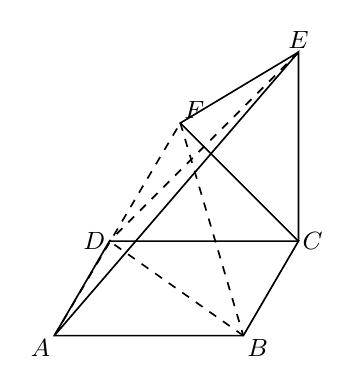
\begin{tikzpicture}[semithick, every node/.style={inner sep=1.2pt, font=\small}]
  \coordinate (A) at (0,0);
  \coordinate (B) at (2.4,0);
  \coordinate (C) at (3.1,1.2);
  \coordinate (D) at (0.7,1.2);
  \coordinate (E) at (3.1,3.6);
  \coordinate (F) at (1.6,2.7);
  % 底面
  \draw (A) -- (B) -- (C) -- (D) -- cycle;
  % 四边形 ACEF
  \draw (A) -- (E) -- (C);
  \draw[dashed] (A) -- (F);
  \draw (E) -- (F) -- (C);
  \draw[dashed] (F) -- (B);
  \draw[dashed] (E) -- (D);
  \draw[dashed] (B) -- (D);
  % 标注
  \node[below left] at (A) {$A$};
  \node[below right] at (B) {$B$};
  \node[right] at (C) {$C$};
  \node[left] at (D) {$D$};
  \node[above] at (E) {$E$};
  \node[above right] at (F) {$F$};
\end{tikzpicture}
\end{center}
\nopagebreak[4]
\end{question}
\begin{question}
\gkti{18}设函数 $f(x)=\dfrac a3x^3+bx^2+cx+d$（$a>0$），且方程 $f'(x)-9x=0$ 的两个根分别为 $1$，$4$。

（1）当 $a=3$ 且曲线 $y=f(x)$ 过原点时，求 $f(x)$ 的解析式；

（2）若 $f(x)$ 在 $(-\infty,+\infty)$ 内无极值点，求 $a$ 的取值范围。

\end{question}
\begin{question}
\gkti{19}已知椭圆 $C$ 的左、右焦点坐标分别是 $(-\sqrt2,0)$，$(\sqrt2,0)$，离心率是 $\dfrac{\sqrt6}3$。直线 $y=t$ 与椭圆 $C$ 交于不同的两点 $M$，$N$，以线段 $MN$ 为直径作圆 $P$，圆心为 $P$。

（1）求椭圆 $C$ 的方程；

（2）若圆 $P$ 与 $x$ 轴相切，求圆心 $P$ 的坐标；

（3）设 $Q(x,y)$ 是圆 $P$ 上的动点，当 $t$ 变化时，求 $y$ 的最大值。

\end{question}
\begin{question}
\gkti{20}已知集合 $S_n=\{X\mid X=(x_1,x_2,\cdots,x_n),\ x_i\in\{0,1\},\ i=1,2,\cdots,n\}$（$n\geqslant2$）。对于 $A=(a_1,a_2,\cdots,a_n)$，$B=(b_1,b_2,\cdots,b_n)\in S_n$，定义 $A$ 与 $B$ 的差为 $A-B=(|a_1-b_1|,|a_2-b_2|,\cdots,|a_n-b_n|)$；$A$ 与 $B$ 之间的距离为 $d(A,B)=\sum\limits_{i=1}^n|a_i-b_i|$。

（1）当 $n=5$ 时，设 $A=(0,1,0,0,1)$，$B=(1,1,1,0,0)$，求 $A-B$，$d(A,B)$；

（2）证明：$\forall A,B,C\in S_n$，有 $A-B\in S_n$，且 $d(A-C,B-C)=d(A,B)$；

（3）证明：$\forall A,B,C\in S_n$，$d(A,B)$，$d(A,C)$，$d(B,C)$ 三个数中至少有一个是偶数。

\end{question}